\documentclass[letterpaper,10pt]{article}

\usepackage{listings}
\usepackage{color}
\usepackage{tikz}

\setlength{\headheight}{0in}
\setlength{\marginparsep}{0in}
\setlength{\footskip}{0in}
\setlength{\headsep}{0in}
\setlength{\marginparwidth}{0in}
\setlength{\marginparpush}{0in}
\setlength{\voffset}{0in}
\setlength{\hoffset}{-1in}
\setlength{\voffset}{-1in}
\setlength{\oddsidemargin}{0.75in}
\setlength{\evensidemargin}{0.75in}
\setlength{\topmargin}{0.75in}
\setlength{\textheight}{9.5in}
\setlength{\textwidth}{7in}
\setlength{\parindent}{0in}
\setlength{\parskip}{10pt} %change this to match font size

\pagestyle{empty}
\definecolor{gray}{gray}{0.75}
\usetikzlibrary{shapes,arrows,calc}
\lstset{numbers=left,backgroundcolor=\color{gray},frame=single}

% define block styles
\tikzstyle{line} = [draw, -latex']
\tikzstyle{block} = [draw, rectangle, text centered, minimum height=2em]
\tikzstyle{mlblock} = [draw, rectangle, text width=10em, text centered, minimum height=2em]
\tikzstyle{decision} = [draw, diamond, text width=4.5em, text centered, node distance=3cm, inner sep=0pt]
\tikzstyle{cloud} = [draw, rectangle, text centered, rounded corners, minimum height=2em]

\begin{document}
    Albert Chang and Nipun Chopra\\
    CSE-380 A6\\
    University at Buffalo\\
    Dr. Kris Schindler\\
    March 1, 2011\\
    \textit{Lab 4 Documentation}

    The objective of Lab 4 was to learn about using the general purpose
    input/output, GPIO, and how to factor code using \textbf{export} and
    \textbf{extern}. There are two parts to the program.

    First the user pushes each of the four push buttons. As the buttons are
    pushed, the corresponding LEDs light up. After each individual button has
    been pushed once, the program moves onto the second part of the program.

    The second part makes use of the UART. The user enters in a hexadecimal,
    0-9, a-f, and A-F, and it is printed on the seven-segment display. Upon
    writting either Q or q, the program quits.

    The user is given feedback by the RGB LED. When the program is waiting for
    push button input, it lights green. When the user pushes a button, it
    lights blue. When it is waiting for UART input, it lights white. Finally,
    when it exits, it lights red.

    Half of the routines were written in the previous labs. Their respective
    flowcharts are shown in Figs. \ref{flo:uart_init}, \ref{flo:chars},
    \ref{flo:output_string}, and \ref{flo:read_string}.

    \begin{figure}[p]
        \begin{center}
    \begin{tikzpicture}[node distance = 3cm, auto]
        \node[cloud] (origin) {Start};
        \node[block, below of=origin, node distance=1.5cm] (enable) {Write 0x5 to PINSEL0 to enable UART0};
        \node[mlblock, below of=enable] (init) {Configure U0LCR:\\%
                                                8-bit word length\\%
                                                1 stop bit\\%
                                                no parity\\%
                                                disable break control\\%
                                                enable access latch};
        \node[block, below of=init] (baud) {Set baud rate to 9600};
        \node[mlblock, below of=baud] (conf) {Configure U0LCR:\\%
                                                8-bit word length\\%
                                                1 stop bit\\%
                                                no parity\\%
                                                disable break control\\%
                                                disable latch access};
        \node[cloud, below of=conf] (stop) {Stop};
        \path[line] (origin) -- (enable);
        \path[line] (enable) -- (init);
        \path[line] (init) -- (baud);
        \path[line] (baud) -- (conf);
        \path[line] (conf) -- (stop);
    \end{tikzpicture}
\end{center}

        \caption{Flowchart of \textit{uart\_init} routine.}
        \label{flo:uart_init}
    \end{figure}

    \begin{figure}[p]
        \begin{minipage}{0.5\linewidth}
            \begin{center}
    \begin{tikzpicture}[node distance = 1.5cm, auto]
        \node[cloud] (origin) {Start};
        \node[decision, below of=origin] (test) {Test THRE in status register};
        \node[block, below of=test, node distance = 3.5cm] (store) {Store byte in transmit register};
        \node[cloud, below of=store] (stop) {Stop};
        \path[line] (origin) -- (test);
        \path[line] (test) -- node [near start] {1} (store);
        \path[line] (test) -| node [near start] {0} +(3,2.25) -- +(0,2.25);
        \path[line] (store) -- (stop);
    \end{tikzpicture}
\end{center}

        \end{minipage}%
        \begin{minipage}{0.5\linewidth}
            \begin{center}
    \begin{tikzpicture}[node distance = 1.5cm, auto]
        \node[cloud] (origin) {Start};
        \node[decision, below of=origin] (test) {Test RDR in status register};
        \node[block, below of=test, node distance = 3.5cm] (read) {Read byte from receive register};
        \node[cloud, below of=read] (stop) {Stop};
        \path[line] (origin) -- (test);
        \path[line] (test) -- node [near start] {1} (read);
        \path[line] (test) -| node [near start] {0} +(3,2) -- +(0,2);
        \path[line] (read) -- (stop);
    \end{tikzpicture}
\end{center}

        \end{minipage}
        \caption{Flowcharts of \textit{output\_char} (left) and \textit{read\_char} (right) routines.}
        \label{flo:chars}
    \end{figure}

    \begin{figure}[p]
        \begin{center}
    \begin{tikzpicture}[node distance = 1.5cm, auto]
        \node[cloud] (origin) {Start};
        \node[block, below of=origin] (read) {Load byte from memory};
        \node[decision, below of=read] (null) {Is it the null character?};
        \node[block, right of=null, node distance=5cm] (output) {Output character};
        \node[cloud, below of=null, node distance=3cm] (stop) {Stop};
        \path[line] (origin) -- (read);
        \path[line] (read) -- (null);
        \path[line] (null) -- node [near start] {no} (output);
        \path[line] (output) |- (read);
        \path[line] (null) -- node [near start] {yes} (stop);
    \end{tikzpicture}
\end{center}

        \caption{Flowchart of \textit{output\_string} routine.}
        \label{flo:output_string}
    \end{figure}

    \begin{figure}[p]
        \begin{center}
    \begin{tikzpicture}[node distance = 1.5cm, auto]
        \node[cloud] (origin) {Start};
        \node[block, below of=origin] (read) {Read from UART};
        \node[block, below of=read] (write) {Output character unconditionally};
        \node[decision, below of=write] (printable) {Is it a printable character?};
        \node[block, below of=printable, node distance=3cm] (store) {Store character into memory};
        \node[decision, below of=store] (cr) {Did the user hit the Enter key?};
        \node[block, below of=cr, node distance=3cm] (null) {Store null character};
        \node[block, below of=null] (nl) {Output a newline};
        \node[cloud, below of=nl] (stop) {Stop};
        \path[line] (origin) -- (read);
        \path[line] (read) -- (write);
        \path[line] (write) -- (printable);
        \path[line] (printable) -| node [near start] {no} +(3,-6) -- (cr);
        \path[line] (printable) -- node [near start] {yes} (store);
        \path[line] (store) -- (cr);
        \path[line] (cr) -| node [near start] {no} +(-4,10.5) -- (read);
        \path[line] (cr) -- node [near start] {yes} (null);
        \path[line] (null) -- (nl);
        \path[line] (nl) -- (stop);
    \end{tikzpicture}
\end{center}

        \caption{Flowchart of \textit{read\_string} routine.}
        \label{flo:read_string}
    \end{figure}

    All of the new routines are linear, simply reading from or writing to
    their respective register. According to the \textit{LPC2138 Education Board
    Users Guide}, the LEDs light when signals are pulled low. So sending a 1
    to them, with IOSET, turns them off, while sending a 0 to them, with IOCLR,
    turns them on.
\end{document}
